\documentclass[10pt,journal,compsoc]{IEEEtran}

\usepackage[T1]{fontenc}
\usepackage{amsmath,amssymb,amsthm}
\usepackage{graphicx}
\usepackage{booktabs}
\usepackage{array}
\usepackage{multirow}
\usepackage{xcolor}
\usepackage{microtype}
\usepackage[hidelinks]{hyperref}
\usepackage{cite}

\graphicspath{{gen/figures/}}
\newtheorem{proposition}{Proposition}
\newtheorem{corollary}{Corollary}
\newcommand{\arm}[1]{\texttt{#1}}
\newcommand{\mnats}{\,mnats}
\newcommand{\eps}{\varepsilon}
% a generated table body; the primitive input keeps the following rule legal inside a tabular
\makeatletter\newcommand{\gen}[1]{\@@input gen/#1.tex }\makeatother

% generated by mvs.paper; do not edit
\newcommand{\warmPasses}{20}
\newcommand{\rewarmSteps}{100}
\newcommand{\horizon}{300}
\newcommand{\evalEvery}{10}
\newcommand{\evalSamples}{512}
\newcommand{\maxSteps}{2000}
\newcommand{\warmupSteps}{100}
\newcommand{\bootDraws}{10000}
\newcommand{\nCells}{540}
\newcommand{\nArms}{15}
\newcommand{\nSeedsMin}{3}
\newcommand{\nSeedsMax}{3}
\newcommand{\seedsXS}{3}
\newcommand{\paramsXS}{0.8}
\newcommand{\seedsS}{3}
\newcommand{\paramsS}{10.7}
\newcommand{\seedsM}{3}
\newcommand{\paramsM}{25.3}
\newcommand{\epsMin}{10.0}
\newcommand{\epsMax}{36.2}
\newcommand{\bandLamMin}{4}
\newcommand{\bandLamMax}{216}
\newcommand{\payFull}{100}
\newcommand{\peakFull}{0.0}
\newcommand{\ratioFull}{0.00}
\newcommand{\lamFull}{0.0}
\newcommand{\regretFull}{0.00}
\newcommand{\inbandFull}{12/12}
\newcommand{\censFull}{0}
\newcommand{\lateFull}{--}
\newcommand{\payWMqeightVlogeight}{50}
\newcommand{\peakWMqeightVlogeight}{2.2}
\newcommand{\ratioWMqeightVlogeight}{0.09}
\newcommand{\lamWMqeightVlogeight}{1.1}
\newcommand{\regretWMqeightVlogeight}{0.12}
\newcommand{\inbandWMqeightVlogeight}{12/12}
\newcommand{\censWMqeightVlogeight}{0}
\newcommand{\lateWMqeightVlogeight}{--}
\newcommand{\payWMVrone}{67}
\newcommand{\peakWMVrone}{4.1}
\newcommand{\ratioWMVrone}{0.17}
\newcommand{\lamWMVrone}{4.4}
\newcommand{\regretWMVrone}{0.23}
\newcommand{\inbandWMVrone}{12/12}
\newcommand{\censWMVrone}{0}
\newcommand{\lateWMVrone}{--}
\newcommand{\payWV}{67}
\newcommand{\peakWV}{6.8}
\newcommand{\ratioWV}{0.29}
\newcommand{\lamWV}{8.2}
\newcommand{\regretWV}{0.72}
\newcommand{\inbandWV}{12/12}
\newcommand{\censWV}{0}
\newcommand{\lateWV}{--}
\newcommand{\payWVsvdfour}{34}
\newcommand{\peakWVsvdfour}{7.9}
\newcommand{\ratioWVsvdfour}{0.33}
\newcommand{\lamWVsvdfour}{8.7}
\newcommand{\regretWVsvdfour}{0.80}
\newcommand{\inbandWVsvdfour}{12/12}
\newcommand{\censWVsvdfour}{0}
\newcommand{\lateWVsvdfour}{--}
\newcommand{\payWEmbV}{34}
\newcommand{\peakWEmbV}{7.4}
\newcommand{\ratioWEmbV}{0.31}
\newcommand{\lamWEmbV}{8.9}
\newcommand{\regretWEmbV}{0.82}
\newcommand{\inbandWEmbV}{12/12}
\newcommand{\censWEmbV}{0}
\newcommand{\lateWEmbV}{--}
\newcommand{\payWVrone}{33}
\newcommand{\peakWVrone}{7.4}
\newcommand{\ratioWVrone}{0.31}
\newcommand{\lamWVrone}{9.1}
\newcommand{\regretWVrone}{0.80}
\newcommand{\inbandWVrone}{12/12}
\newcommand{\censWVrone}{0}
\newcommand{\lateWVrone}{--}
\newcommand{\payWbfsixteenVrone}{17}
\newcommand{\peakWbfsixteenVrone}{7.5}
\newcommand{\ratioWbfsixteenVrone}{0.31}
\newcommand{\lamWbfsixteenVrone}{9.1}
\newcommand{\regretWbfsixteenVrone}{0.85}
\newcommand{\inbandWbfsixteenVrone}{12/12}
\newcommand{\censWbfsixteenVrone}{0}
\newcommand{\lateWbfsixteenVrone}{--}
\newcommand{\payWM}{67}
\newcommand{\peakWM}{1469.1}
\newcommand{\ratioWM}{69.26}
\newcommand{\lamWM}{634.6}
\newcommand{\regretWM}{177.36}
\newcommand{\inbandWM}{0/12}
\newcommand{\censWM}{9}
\newcommand{\lateWM}{40}
\newcommand{\payWZero}{33}
\newcommand{\peakWZero}{271.3}
\newcommand{\ratioWZero}{11.40}
\newcommand{\lamWZero}{56.8}
\newcommand{\regretWZero}{19.80}
\newcommand{\inbandWZero}{3/12}
\newcommand{\censWZero}{3}
\newcommand{\lateWZero}{75}
\newcommand{\payWFresh}{33}
\newcommand{\peakWFresh}{105.7}
\newcommand{\ratioWFresh}{4.38}
\newcommand{\lamWFresh}{26.4}
\newcommand{\regretWFresh}{6.40}
\newcommand{\inbandWFresh}{5/12}
\newcommand{\censWFresh}{3}
\newcommand{\lateWFresh}{25}
\newcommand{\payWRewarm}{33}
\newcommand{\peakWRewarm}{19.8}
\newcommand{\ratioWRewarm}{0.83}
\newcommand{\lamWRewarm}{35.3}
\newcommand{\regretWRewarm}{2.88}
\newcommand{\inbandWRewarm}{11/12}
\newcommand{\censWRewarm}{1}
\newcommand{\lateWRewarm}{--}
\newcommand{\payWWarmv}{33}
\newcommand{\peakWWarmv}{9.5}
\newcommand{\ratioWWarmv}{0.40}
\newcommand{\lamWWarmv}{27.2}
\newcommand{\regretWWarmv}{0.68}
\newcommand{\inbandWWarmv}{10/12}
\newcommand{\censWWarmv}{0}
\newcommand{\lateWWarmv}{55}
\newcommand{\payWMWarm}{67}
\newcommand{\peakWMWarm}{13.1}
\newcommand{\ratioWMWarm}{0.55}
\newcommand{\lamWMWarm}{23.7}
\newcommand{\regretWMWarm}{0.40}
\newcommand{\inbandWMWarm}{9/12}
\newcommand{\censWMWarm}{0}
\newcommand{\lateWMWarm}{20}
\newcommand{\payWWarm}{33}
\newcommand{\peakWWarm}{204.0}
\newcommand{\ratioWWarm}{8.44}
\newcommand{\lamWWarm}{64.2}
\newcommand{\regretWWarm}{15.15}
\newcommand{\inbandWWarm}{4/12}
\newcommand{\censWWarm}{3}
\newcommand{\lateWWarm}{30}
\newcommand{\forkList}{200, 600, 1200, 1700}
\newcommand{\sizeQXS}{0.07}
\newcommand{\sizeVXS}{0.20}
\newcommand{\sizeRankXS}{0.22}
\newcommand{\sizeRankBfXS}{0.26}
\newcommand{\sizeMXS}{42.10}
\newcommand{\sizeZeroXS}{2.51}
\newcommand{\sizeFreshXS}{1.08}
\newcommand{\sizeRewarmXS}{0.71}
\newcommand{\sizeWarmvXS}{0.22}
\newcommand{\sizeWarmXS}{3.72}
\newcommand{\sizeQS}{0.02}
\newcommand{\sizeVS}{0.30}
\newcommand{\sizeRankS}{0.31}
\newcommand{\sizeRankBfS}{0.31}
\newcommand{\sizeMS}{102.63}
\newcommand{\sizeZeroS}{9.58}
\newcommand{\sizeFreshS}{4.11}
\newcommand{\sizeRewarmS}{0.89}
\newcommand{\sizeWarmvS}{0.34}
\newcommand{\sizeWarmS}{9.23}
\newcommand{\sizeQM}{0.09}
\newcommand{\sizeVM}{0.29}
\newcommand{\sizeRankM}{0.31}
\newcommand{\sizeRankBfM}{0.31}
\newcommand{\sizeMM}{69.26}
\newcommand{\sizeZeroM}{11.40}
\newcommand{\sizeFreshM}{4.38}
\newcommand{\sizeRewarmM}{0.83}
\newcommand{\sizeWarmvM}{0.40}
\newcommand{\sizeWarmM}{8.44}
\newcommand{\epsEarly}{24.8}
\newcommand{\peakEarlyQ}{6.1}
\newcommand{\ratioEarlyQ}{0.25}
\newcommand{\peakEarlyV}{18.5}
\newcommand{\ratioEarlyV}{0.75}
\newcommand{\peakEarlyRank}{21.6}
\newcommand{\ratioEarlyRank}{0.87}
\newcommand{\peakEarlyRankBf}{21.7}
\newcommand{\ratioEarlyRankBf}{0.88}
\newcommand{\peakEarlyM}{1539.2}
\newcommand{\ratioEarlyM}{62.14}
\newcommand{\peakEarlyZero}{750.1}
\newcommand{\ratioEarlyZero}{30.28}
\newcommand{\peakEarlyFresh}{347.9}
\newcommand{\ratioEarlyFresh}{14.04}
\newcommand{\peakEarlyRewarm}{56.9}
\newcommand{\ratioEarlyRewarm}{2.30}
\newcommand{\peakEarlyWarmv}{28.5}
\newcommand{\ratioEarlyWarmv}{1.15}
\newcommand{\peakEarlyWarm}{663.1}
\newcommand{\ratioEarlyWarm}{26.77}
\newcommand{\epsLate}{16.4}
\newcommand{\peakLateQ}{0.1}
\newcommand{\ratioLateQ}{0.01}
\newcommand{\peakLateV}{0.1}
\newcommand{\ratioLateV}{0.01}
\newcommand{\peakLateRank}{0.1}
\newcommand{\ratioLateRank}{0.01}
\newcommand{\peakLateRankBf}{0.2}
\newcommand{\ratioLateRankBf}{0.01}
\newcommand{\peakLateM}{214.5}
\newcommand{\ratioLateM}{13.05}
\newcommand{\peakLateZero}{9.3}
\newcommand{\ratioLateZero}{0.57}
\newcommand{\peakLateFresh}{2.0}
\newcommand{\ratioLateFresh}{0.12}
\newcommand{\peakLateRewarm}{1.5}
\newcommand{\ratioLateRewarm}{0.09}
\newcommand{\peakLateWarmv}{0.4}
\newcommand{\ratioLateWarmv}{0.02}
\newcommand{\peakLateWarm}{1.2}
\newcommand{\ratioLateWarm}{0.07}
\newcommand{\bytesWorstPct}{0.04}
\newcommand{\overshootA}{2.13}
\newcommand{\overshootAtA}{13}
\newcommand{\overshootB}{6.57}
\newcommand{\overshootAtB}{12}
\newcommand{\firstNoiseA}{4.4}
\newcommand{\excessZerosA}{109}
\newcommand{\firstNoiseB}{13.8}
\newcommand{\excessZerosB}{1292}
\newcommand{\firstNoiseC}{1.9}
\newcommand{\excessZerosC}{14}
\newcommand{\excessFreshA}{16}
\newcommand{\deficitM}{2.5}
\newcommand{\traceScale}{gpt-s}
\newcommand{\traceSeeds}{2}
\newcommand{\traceSteps}{150}
\newcommand{\traceZeroOne}{4.59}
\newcommand{\traceZeroTen}{2.67}
\newcommand{\traceZeroHundred}{1.20}
\newcommand{\traceZeroOneEarly}{6.12}
\newcommand{\traceZeroTenEarly}{3.51}
\newcommand{\traceZeroHundredEarly}{1.07}
\newcommand{\traceFreshOne}{4.62}
\newcommand{\traceFreshTen}{1.34}
\newcommand{\traceFreshHundred}{0.99}
\newcommand{\traceFreshOneEarly}{6.62}
\newcommand{\traceFreshTenEarly}{1.92}
\newcommand{\traceFreshHundredEarly}{0.99}
\newcommand{\traceVOne}{0.45}
\newcommand{\traceVTen}{0.94}
\newcommand{\traceVHundred}{1.00}
\newcommand{\traceVOneEarly}{0.68}
\newcommand{\traceVTenEarly}{0.95}
\newcommand{\traceVHundredEarly}{1.02}
\newcommand{\traceWarmOne}{1.84}
\newcommand{\traceWarmTen}{1.24}
\newcommand{\traceWarmHundred}{1.01}
\newcommand{\traceWarmOneEarly}{4.79}
\newcommand{\traceWarmTenEarly}{2.37}
\newcommand{\traceWarmHundredEarly}{0.72}
\newcommand{\traceRankOne}{0.46}
\newcommand{\traceRankTen}{0.94}
\newcommand{\traceRankHundred}{1.00}
\newcommand{\traceRankOneEarly}{0.67}
\newcommand{\traceRankTenEarly}{0.94}
\newcommand{\traceRankHundredEarly}{1.00}
\newcommand{\traceQOne}{1.00}
\newcommand{\traceQTen}{1.00}
\newcommand{\traceQHundred}{1.00}
\newcommand{\traceQOneEarly}{1.00}
\newcommand{\traceQTenEarly}{1.00}
\newcommand{\traceQHundredEarly}{1.00}
\newcommand{\predZeroOne}{4.36}
\newcommand{\predZeroTen}{3.03}
\newcommand{\predZeroHundred}{1.26}
\newcommand{\predFreshOne}{4.36}
\newcommand{\predFreshTen}{1.44}
\newcommand{\predFreshHundred}{1.00}
\newcommand{\predVOne}{0.44}
\newcommand{\predVTen}{0.94}
\newcommand{\predVHundred}{1.00}
\newcommand{\llamaParams}{6.74}
\newcommand{\llamaFullGB}{80.9}
\newcommand{\llamaFullDrain}{64.7}
\newcommand{\llamaQGB}{40.7}
\newcommand{\llamaQDrain}{32.6}
\newcommand{\llamaRankGB}{27.0}
\newcommand{\llamaRankDrain}{21.6}
\newcommand{\llamaRankBfGB}{13.5}
\newcommand{\llamaRankBfDrain}{10.8}
\newcommand{\latReps}{20}
\newcommand{\mbFull}{304}
\newcommand{\drainFull}{580}
\newcommand{\restoreFull}{427}
\newcommand{\encodeFull}{0}
\newcommand{\drainQ}{442}
\newcommand{\restoreQ}{248}
\newcommand{\encodeQ}{90}
\newcommand{\drainRank}{219}
\newcommand{\restoreRank}{157}
\newcommand{\encodeRank}{3}
\newcommand{\drainRankBf}{127}
\newcommand{\restoreRankBf}{106}
\newcommand{\encodeRankBf}{4}
\newcommand{\drainSvd}{1052}
\newcommand{\restoreSvd}{131}
\newcommand{\encodeSvd}{839}
\newcommand{\drainWarm}{209}
\newcommand{\restoreWarm}{5742}
\newcommand{\encodeWarm}{0}
\newcommand{\devWorstXpuAmp}{0.52}
\newcommand{\devWorstCpuFp}{0.00}
\newcommand{\devWorstXpuFp}{0.31}
\newcommand{\stepZero}{5.0}
\newcommand{\cosZero}{0.35}
\newcommand{\mnormZero}{0.0}
\newcommand{\verrZero}{100}
\newcommand{\stepFresh}{5.2}
\newcommand{\cosFresh}{0.35}
\newcommand{\mnormFresh}{0.0}
\newcommand{\verrFresh}{100}
\newcommand{\stepWarm}{2.6}
\newcommand{\cosWarm}{0.22}
\newcommand{\mnormWarm}{4.0}
\newcommand{\verrWarm}{23}
\newcommand{\stepM}{175.9}
\newcommand{\cosM}{0.22}
\newcommand{\mnormM}{1.0}
\newcommand{\verrM}{100}
\newcommand{\stepRank}{0.5}
\newcommand{\cosRank}{0.44}
\newcommand{\mnormRank}{0.0}
\newcommand{\verrRank}{8}
\newcommand{\stepV}{0.5}
\newcommand{\cosV}{0.45}
\newcommand{\mnormV}{0.0}
\newcommand{\verrV}{0}
\newcommand{\chaosGpuGoodput}{0.719}
\newcommand{\chaosGpuWall}{384}
\newcommand{\chaosGpuWallCtrl}{359}
\newcommand{\chaosGpuEvents}{3}
\newcommand{\chaosGpuMttr}{5.257}
\newcommand{\chaosGpuRedone}{1}
\newcommand{\chaosGpuGap}{1.8}
\newcommand{\chaosResizeGoodput}{0.979}
\newcommand{\chaosResizeWall}{930}
\newcommand{\chaosResizeWallCtrl}{996}
\newcommand{\chaosResizeEvents}{3}
\newcommand{\chaosResizeMttr}{6.788}
\newcommand{\chaosResizeRedone}{1}
\newcommand{\chaosResizeGap}{13.7}

% Numbers that come from optional experiments. gen/numbers.tex defines them when the experiment was run; a draft built
% before that shows a visible marker instead of failing.
\newcommand{\pending}{\textcolor{red}{n/a}}
\makeatletter
\@for\name:=latReps,drainFull,drainQ,drainRank,drainWarm,restoreFull,restoreQ,restoreRank,%
restoreWarm,devWorstCpuFp,devWorstXpuFp,devWorstXpuAmp,devWorstCudaFp,devWorstCudaAmp,chaosGpuGoodput,chaosGpuMttr,%
chaosGpuRedone,chaosGpuGap,chaosResizeGoodput,chaosResizeMttr,chaosResizeRedone,chaosResizeGap,stepZero,stepFresh,%
stepWarm,stepM,stepRank,stepV,cosZero,cosFresh,cosWarm,cosM,cosRank,cosV,mnormZero,mnormFresh,mnormWarm,mnormM,%
mnormRank,mnormV,verrZero,verrFresh,verrWarm,verrM,verrRank,verrV,traceScale,traceSeeds,traceSteps,%
ratioWM,ratioWZero,peakWM,peakWZero,inbandWM,inbandWZero,censWM,censWZero,regretWM,regretWZero,lamWM,lamWZero%
\do{\@ifundefined{\name}{\expandafter\let\csname\name\endcsname\pending}{}}
\makeatother


\begin{document}

\title{Minimum Viable State: What Adam Must Carry\\Across a Preemption}

\author{Ritesh~Roshan~Sahoo%
\IEEEcompsocitemizethanks{\IEEEcompsocthanksitem R.~R.~Sahoo is with the School of Artificial Intelligence, Amrita Vishwa Vidyapeetham, Faridabad, Haryana, India.\protect\\
E-mail: riteshroshansahoo01@gmail.com.}}

\markboth{}{Sahoo: Minimum Viable State: What Adam Must Carry Across a Preemption}

\IEEEtitleabstractindextext{%
\begin{abstract}
Training jobs on preemptible machines get a notice of thirty seconds to two minutes before the machine is reclaimed.
Every published elastic or spot training system uses that window to move the complete optimizer state, which for Adam is
three times the size of the model, and treats the cost of recovery as a constant. This paper measures which parts of
that state have to cross. A training run is interrupted at a chosen step, resumed from \nArms{} different payloads, and
compared with a bit-identical uninterrupted control over \nCells{} migrations, three model sizes and up to \nSeedsMax{}
seeds, against a noise floor set by the spread between seeds. Three results follow. Quantised moments at half the bytes
are indistinguishable from the full state. A row-and-column sketch of the second moment, with the first moment dropped,
cuts the payload to a third, or a sixth with half-precision weights, and stays inside the noise floor. Dropping both
moments does not, and the damage is concentrated early in training; the two repairs in common use, resetting the step
counter and re-estimating the moments from fresh gradients, are the two worst options measured. A short analysis
predicts the size and duration of each transient from the two decay rates alone and agrees with measured update sizes.
Payload sizes are measured from the serialised bytes, drain and restore times are timed stage by stage, and the same
payloads are resumed on a CPU, a discrete GPU and an integrated GPU. A cost model turns the measurements into a rule
for what to send inside a given notice window.

\end{abstract}
\begin{IEEEkeywords}
Elastic training, spot instances, preemption, checkpointing, optimizer state, Adam, state migration, fault tolerance, cloud economics.
\end{IEEEkeywords}}

\maketitle
\IEEEdisplaynontitleabstractindextext
\IEEEpeerreviewmaketitle

\section{Introduction}
\label{sec:intro}

\IEEEPARstart{P}{reemptible} capacity is the cheapest way to rent an accelerator and the least dependable. A spot
instance is reclaimed with a warning of two minutes on one large cloud and at most thirty seconds on two
others~\cite{wu2024cantbelate,lee2022spotlake}. In that window a training job has to get its state off the machine. For
a model trained with Adam~\cite{kingma2015adam,loshchilov2019adamw} the state is the weights and two moment tensors of
the same shape, twelve bytes per parameter in single precision. A \llamaParams{}-billion-parameter model therefore owns
\llamaFullGB{}\,GB of state, which takes \llamaFullDrain{}\,s to drain over a 10\,Gb/s link before any serialisation
cost: inside a two-minute notice, outside a thirty-second one.

The systems that keep training alive on such machines differ in almost everything except this. They re-plan pipelines
when workers vanish~\cite{athlur2022varuna,thorpe2023bamboo,jang2023oobleck,duan2024parcae}, replicate state to
peers~\cite{wang2023gemini}, rebuild it from mirrored gradients~\cite{bhardwaj2025checkmate}, migrate it directly
between nodes~\cite{liu2026etc}, or snapshot the whole device~\cite{stoyanov2025criugpu,wei2025phoenixos}. All of them
move the weights and both moments in full. The most recent migration system states the assumption outright: ``it is
necessary to migrate model parameters, optimizer states and other states''~\cite{liu2026etc}. The schedulers that decide
when to use spot capacity then fold everything that happens at a switch into one constant, the changeover
delay~\cite{wu2024cantbelate}.

Work on optimizers points the other way. Adafactor trains with only the row and column sums of the second
moment~\cite{shazeer2018adafactor}; later work removes or compresses most of it for the whole
run~\cite{zhang2025adammini,kalra2025slimadam} and stores both moments in eight or four
bits~\cite{dettmers2022eightbit,li2023fourbit}. If a run can live with a coarse second moment at every step, it can
presumably survive receiving a coarse one once. Nobody has measured that. The question is not whether the state can be
made smaller, which checkpoint compression already answers~\cite{li2024excp,zhang2026guarded}, but which of it has to
exist on the wire at all, and what is paid in training progress for each part left behind.

This paper answers that question by experiment. A run is stopped at step $T$, its state is reduced according to a
\emph{strategy}, and training resumes from what is left. The resumed run is compared, step by step, with a control that
was never interrupted. Because data order, dropout masks and the learning-rate schedule are all pure functions of the
step index, the control and the resumed run differ in exactly one thing, the state that crossed, and a resume from the
full state reproduces the control bit for bit. Because two runs that differ only in their seed also drift apart, every
gap is read against that spread, the \emph{seed band}; a migrated run that stays inside it cannot be told from a
different seed of the same job.

The contributions are as follows.

\begin{itemize}
\item \textbf{A controlled ablation of optimizer state at a migration boundary.} \nArms{} payload strategies, from the
full state down to the weights alone, are evaluated over \nCells{} migrations on three model sizes, four points in
training and up to \nSeedsMax{} seeds, with bootstrap intervals over seeds and censored recovery times
(Sections~\ref{sec:setup} and~\ref{sec:results}).
\item \textbf{An account of the arrival transient.} With both moments zeroed, the first update is not small, as is
sometimes assumed, but about $\sqrt{(1-\beta_1^2)/(1-\beta_2)}$ times the steady one, and it decays on the horizon of
the second moment if the step counter is kept and of the first if it is reset. The closed forms agree with measured
update sizes, and explain why the first moment may be dropped, why the second may be sketched, and why a first moment
re-estimated at the destination is harmful (Section~\ref{sec:transient}).
\item \textbf{Measured bytes and latency.} Payload sizes are taken from the serialised bundle and agree with the
analytic count to within \bytesWorstPct\% ; drain and restore are timed per stage over repeated rounds
(Section~\ref{sec:results}).
\item \textbf{Migration across device classes.} The same payload is resumed on a CPU, a discrete GPU and an integrated
GPU of a different vendor, and the gap between devices is itself measured against the seed band
(Section~\ref{sec:device}).
\item \textbf{A policy.} A cost model takes the measured curve, a notice window, a bandwidth and a price, and returns the
cheapest strategy that fits (Section~\ref{sec:policy}). Its outputs for models larger than those trained here are
extrapolations and are labelled as such.
\end{itemize}

The experiments run on one laptop with models of \paramsXS{} to \paramsM{} million parameters, and that limit is
stated wherever it matters. What the paper offers at that scale is a method, a noise floor and a set of mechanisms that
make predictions; Section~\ref{sec:limits} lists what remains to be checked on a real cluster.

\section{Background and Related Work}
\label{sec:related}

\subsection{Adam and its state}

Adam~\cite{kingma2015adam} keeps, for every parameter, an exponential average of the gradient and of its square. With
gradient $g_t$ at optimizer step $t$,
\begin{align}
m_t &= \beta_1 m_{t-1} + (1-\beta_1)\, g_t, \label{eq:m}\\
v_t &= \beta_2 v_{t-1} + (1-\beta_2)\, g_t^2, \label{eq:v}\\
\theta_t &= \theta_{t-1} - \eta_t\, \frac{m_t/(1-\beta_1^{t})}{\sqrt{v_t/(1-\beta_2^{t})} + \epsilon},  \label{eq:step}
\end{align}
with decoupled weight decay in AdamW~\cite{loshchilov2019adamw}. The state of a run is $(\theta, m, v)$, the step
count $t$ that enters the two bias corrections, and a few scalars. The first moment averages over a horizon of about
$1/(1-\beta_1)$ steps, ten at the usual $\beta_1 = 0.9$; the second over $1/(1-\beta_2)$, a hundred to a thousand.
The moments are updated \emph{before} the step is taken, so a moment that arrives as zero is already partly refilled
when it is first used. Section~\ref{sec:transient} depends on this ordering.

\subsection{Training on preemptible and elastic resources}

Varuna~\cite{athlur2022varuna}, Bamboo~\cite{thorpe2023bamboo}, Oobleck~\cite{jang2023oobleck},
Parcae~\cite{duan2024parcae}, ReCycle~\cite{gandhi2024recycle}, Lazarus~\cite{wu2024lazarus} and TrainMover~\cite{lao2024trainmover} keep a pipeline-parallel
job running as workers disappear, by re-planning, redundant computation or replicated stages. Parcae keeps a CPU-side
copy of ``parameters and optimizer states'' so that a preempted worker's state survives~\cite{duan2024parcae}.
Elastic schedulers such as Pollux~\cite{qiao2021pollux} and EasyScale~\cite{li2023easyscale} resize jobs on shared
clusters; EasyScale requires the resized job to reproduce the fixed-size one bit for bit, the standard we adopt
for our control. ETC~\cite{liu2026etc} moves state directly between nodes without a checkpoint; Singularity~\cite{shukla2022singularity}, CRIUgpu~\cite{stoyanov2025criugpu} and
PhoenixOS~\cite{wei2025phoenixos} snapshot the device transparently, which carries at least the resident sixteen bytes
per parameter. On the buying side, SkyPilot~\cite{yang2023skypilot}, Can't Be Late~\cite{wu2024cantbelate} and
SkyNomad~\cite{li2026skynomad} choose between spot and on-demand capacity and between regions; they model recovery as a
fixed delay or a fixed migration cost. In every one of these systems the optimizer state is cargo. None varies what is
carried, so none can say what a smaller cargo costs.

\subsection{Checkpointing}

CheckFreq~\cite{mohan2021checkfreq} tunes how often to checkpoint; Gemini~\cite{wang2023gemini},
Just-in-Time checkpointing~\cite{gupta2024jit}, Swift~\cite{zhong2024swift}, Checkmate~\cite{bhardwaj2025checkmate} and
DataStates-LLM~\cite{maurya2026datastates} make saving or recovering faster while preserving the full state.
A second line makes checkpoints smaller: Check-N-Run~\cite{eisenman2022checknrun} and
Inshrinkerator~\cite{agrawal2024inshrinkerator} store them lossily, ExCP~\cite{li2024excp} prunes weights and moments
jointly, and MoC-System~\cite{cai2025moc} and MoEvement~\cite{gandhi2026moevement} save only some experts of a
mixture-of-experts model at each checkpoint, the nearest precedent for partial state. These papers report compression
ratio against final accuracy after one or more lossy restores. Their concern is the size of what is stored; the
transient that follows a restore, which decides whether a migration is worth making, is not resolved.
Kokolis et al.~\cite{kokolis2025reliability} supply the reliability data and the effective-training-time ratio in which
such costs are counted at scale.

\subsection{Smaller optimizer state}

Adafactor~\cite{shazeer2018adafactor} replaces $v$ for a matrix parameter by its row and column sums.
Adam-mini~\cite{zhang2025adammini} and SlimAdam~\cite{kalra2025slimadam} show that most per-coordinate second moments
can be shared within blocks; SlimAdam finds that embedding matrices resist this along the vocabulary dimension, which
is why we test a strategy that keeps embedding moments exact. Eight-bit and four-bit
optimizers~\cite{dettmers2022eightbit,li2023fourbit} store quantised moments throughout training. All of these keep the
reduced state for the whole run and tune for it. Our question is different. A run trained with exact Adam is handed
a reduced state \emph{once}, and has to carry on.

\subsection{Warm-up, bias correction and restarts}

A freshly initialised Adam takes oversized steps, which is what learning-rate warm-up
compensates~\cite{liu2020radam,ma2021untunedwarmup,kalra2024warmup}; bias correction can be read as an implicit
schedule~\cite{laing2025biascorrection}. Adaptive methods also run at the edge of stability, where the gradient
oscillates across sharp directions~\cite{cohen2022aeos}; Section~\ref{sec:transient} uses that fact. Resetting Adam on
purpose helps in reinforcement learning, where the objective changes~\cite{asadi2023resetting}; here the objective is
stationary and nothing in the moments is stale.

\subsection{Concurrent work}

Two preprints are closest. Mitra~\cite{mitra2026orbittrace} studies training under scheduled interruptions and reports
that a weights-only checkpoint costs final perplexity and accuracy relative to a full one, and that rebuilding a decayed
first moment recovers about a fifth of the penalty, not robustly across seeds. That study measures end-of-run quality;
it does not separate the two moments, account for bytes or resolve the transient, and its restarts change data order.
Zhang et al.~\cite{zhang2026guarded} compress both moments under a bound on the first restored update and cut moment
payloads by about 70\%; they do not drop or rebuild a moment. We use their first-update criterion as a
diagnostic (Section~\ref{sec:diag}), and the quantised strategy below occupies the same point on the trade-off curve.
Relative to both, we add the step-resolved measurement against a deterministic control and a noise
floor, the separation of $m$ from $v$ at equal bytes, the analysis of why each transient has the shape it has, and the
conversion of the result into a migration decision. Table~\ref{tab:position} sets the closest work side by side.

\begin{table*}[t]
\caption{The work this paper builds on, by what state each moves when a job is interrupted and what each measures.}
\label{tab:position}
\centering
\footnotesize
\begin{tabular}{@{}>{\raggedright}p{0.15\textwidth}>{\raggedright}p{0.22\textwidth}>{\raggedright}p{0.25\textwidth}>{\raggedright\arraybackslash}p{0.30\textwidth}@{}}
\toprule
Work & Purpose & State that moves & What is measured \\
\midrule
Parcae~\cite{duan2024parcae} & spot training, proactive re-planning & full; CPU-side copy of parameters and optimizer states & throughput and cost on a replayed spot trace \\\addlinespace[2pt]
Can't Be Late~\cite{wu2024cantbelate} & spot or on-demand under a deadline & not modelled; one constant changeover delay & cost saving on availability traces \\\addlinespace[2pt]
EasyScale~\cite{li2023easyscale} & elastic resizing & full & bitwise equality with the fixed-size run \\\addlinespace[2pt]
ETC~\cite{liu2026etc} & migration without a checkpoint & full, peer to peer & migration overhead \\\addlinespace[2pt]
Checkmate~\cite{bhardwaj2025checkmate} & checkpointing by gradient replication & full, replayed on a shadow cluster & repeated work per failure, throughput \\\addlinespace[2pt]
CRIUgpu~\cite{stoyanov2025criugpu} & transparent device snapshot & all device memory & checkpoint and restore time \\\addlinespace[2pt]
ExCP~\cite{li2024excp} & checkpoint compression & pruned four-bit weights and moments & final accuracy after restores \\\addlinespace[2pt]
MoEvement~\cite{gandhi2026moevement} & sparse checkpoints for mixtures of experts & a subset of experts per checkpoint & checkpoint and recovery overhead \\\addlinespace[2pt]
Zhang et al.~\cite{zhang2026guarded} & guarded moment compression & weights and log-coded moments & first-update error, loss after 100 updates \\\addlinespace[2pt]
Mitra~\cite{mitra2026orbittrace} & training under scheduled interruptions & weights, or weights and a decayed $m$ & final perplexity and accuracy \\
\midrule
This paper & ablation at the migration boundary & \nArms{} payloads, from full to weights alone & held-out loss at every step against a bit-identical control and a seed band; measured bytes and latency \\
\bottomrule
\end{tabular}
\end{table*}

Seed-to-seed variation is large enough to matter for any such comparison~\cite{summers2021nondeterminism,
bouthillier2021variance,vanderwal2025polypythias}, and results are not guaranteed to reproduce across device
types~\cite{pytorch2026randomness,pham2020variance,zhuang2021randomness}; both facts shape the method that follows.

\section{Payload Strategies}
\label{sec:method}

\subsection{What a migration carries}

A migration is a function from the state of the source to the state the destination starts with. It is described by
a \emph{strategy}, a tuple $(c_\theta, c_m, c_v, \rho)$: a codec for the weights, a codec for each moment or nothing if
that moment is left behind, and a rule $\rho$ that says what the destination does about what is missing. The step
index, Adam's step counter, the model's non-trainable buffers and a fingerprint of the configuration always travel;
together they are a few hundred bytes plus the buffers. Table~\ref{tab:bytes} lists the strategies studied.

\textbf{Codecs.} \texttt{fp32} sends a tensor as it is and \texttt{bf16} rounds it to sixteen bits. \texttt{q8} is a
block-wise linear quantiser: each block of 256 values is scaled by its largest magnitude and stored as signed bytes with
one scale per block. \texttt{log8} is its counterpart for the non-negative second moment, which spans many orders of
magnitude within one tensor: the logarithm of each positive entry is quantised to 254 levels between the block's
smallest and largest, and the code zero is kept for exact zeros so that a coordinate that never received gradient
stays at zero. \texttt{rank1} sends, for a tensor reshaped to a matrix $V \in \mathbb{R}^{p \times q}$, only its row
sums $r$ and column sums $c$, and the destination rebuilds $\hat V = r c^{\top} / \sum_i r_i$. This is the Adafactor
estimator~\cite{shazeer2018adafactor}, applied once at the boundary; it is non-negative by construction, so no entry of
the rebuilt second moment can reach the square root with the wrong sign. Vectors are sent whole. \texttt{rank1e} does
the same but sends embedding and output-projection moments exactly, since their rows receive gradient only when their
token is sampled. \texttt{svd}$k$ sends a rank-$k$ factorisation of $\sqrt{V}$ and squares the product at the
destination, which is again non-negative.

\textbf{Reconstruction.} The rule $\rho$ takes one of six values. \texttt{none} applies when both moments arrive.
\texttt{zeros} sets a missing moment to zero and keeps the step counter. \texttt{fresh} zeroes both moments and resets
the counter, which is what constructing a new optimizer does. \texttt{rewarm} does the same and also ramps the learning
rate linearly from zero to its scheduled value over $\rewarmSteps$ steps. \texttt{warm} and \texttt{warmv} spend
$\warmPasses$ forward-backward passes at the destination, on batches drawn from a stream that training never uses,
with the weights held fixed, and install the bias-corrected averages of $g$ and $g^2$ as moments; \texttt{warm}
rebuilds whichever moment is missing and \texttt{warmv} rebuilds only $v$ and leaves $m$ at zero. These passes cost
compute at the destination and no bytes.

The strategies fall into four families: both moments carried (exactly, quantised, or with $v$ sketched), $m$ dropped,
$v$ dropped, and both dropped. \arm{w\_v} and \arm{w\_m} cost the same bytes and differ only in which moment they keep;
\arm{w\_zero} and \arm{w\_fresh} carry the same bytes and differ only in the counter.

\begin{table}[t]
\caption{Strategies and their payloads in bytes per parameter at \paramsM{}M parameters. Analytic sizes are computed
from tensor shapes; measured sizes are the serialised bundle, including header, padding and checksums.}
\label{tab:bytes}
\centering
\footnotesize
\setlength{\tabcolsep}{3.2pt}
\begin{tabular}{@{}lllllrrr@{}}
\toprule
Strategy & $c_\theta$ & $c_m$ & $c_v$ & $\rho$ & Analytic & Measured & $\Delta$\,\% \\
\midrule
\gen{tab_bytes}
\bottomrule
\end{tabular}
\end{table}

\subsection{Wire format and byte accounting}

A payload is one self-describing bundle: a short magic string and version, a JSON header that names every tensor with
its codec, shape, offset and CRC-32, and the tensor blobs aligned to 64 bytes. The header carries the strategy, the
step, the Adam counter and the configuration fingerprint, and the destination reports a bundle whose fingerprint
differs from its own configuration. Files are written to a temporary name, flushed to stable storage and renamed, so that
a process killed while draining leaves the previous payload or the complete new one. A single module owns
serialisation, and every size reported in this paper is the length of the bundle it produced. Table~\ref{tab:bytes}
compares those lengths with the count obtained from tensor shapes alone; the largest disagreement is
\bytesWorstPct\%, which is the header and alignment.

Moving a payload is timed in nine stages: encode, device-to-host copy, serialise and write at the source; read,
deserialise, host-to-device copy, decode and rebuild at the destination. The first four are the \emph{drain}, which must
finish inside the notice window; the last five are the \emph{restore}.

\subsection{Runtime}

The runtime that uses these payloads is small. Each rank watches for a preemption notice from any of four sources: a
termination signal, a sentinel file, and the instance-metadata endpoints of two clouds. At the top of every step the
ranks agree on whether anyone has been notified with one max-reduction, so that all of them stop at the same step. Rank
zero then drains the configured strategy and the group exits with a distinguished status. A launcher restarts the group,
at the same or a different size, from the newest complete payload; a periodic checkpoint, itself written with one of
the strategies, covers failures that arrive without notice. Collectives use the Gloo backend so that the same code runs
on CPUs and on a single GPU.

Because batches are a function of the global step rather than of loader state (Section~\ref{sec:determinism}), a
resized group sees the same data as the original, and nothing about the data pipeline has to be checkpointed.

\section{The Arrival Transient}
\label{sec:transient}

Before looking at any data we can work out what should happen in the first steps after a reduced state arrives.
It takes nothing more than \eqref{eq:m}--\eqref{eq:step}, and the answer tells us which strategies are worth running
and what to expect from each. Number the steps after
arrival $k = 1, 2, \dots$ and consider one coordinate whose gradient over this short window has mean $\mu$ and variance
$\sigma^2$, with independent noise from step to step. Let $R(k)$ be the root-mean-square size of the update at step
$k$ divided by its size in the uninterrupted run. Two limits bracket the behaviour: a coordinate dominated by noise
($\mu = 0$) and one dominated by signal ($\sigma = 0$). In the uninterrupted run the noise-dominated update has
size $\eta\sqrt{(1-\beta_1)/(1+\beta_1)}$, about $0.23\,\eta$ at $\beta_1 = 0.9$, and the signal-dominated one has
size $\eta$. The Adam counter at arrival is large, so that both bias corrections equal one unless the counter is reset.

\begin{proposition}[Size of the arrival transient]
\label{prop:transient}
Approximating $v$ by its expectation, the update inflation $R(k)$ is as follows.

\smallskip
\noindent\small\setlength{\tabcolsep}{3pt}\begin{tabular}{@{}lll@{}}
\toprule
State on arrival & Noise-dominated & Signal-dominated \\
\midrule
$m = v = 0$, counter kept & $\sqrt{\dfrac{1-\beta_1^{2k}}{1-\beta_2^{k}}}$ & $\dfrac{1-\beta_1^{k}}{\sqrt{1-\beta_2^{k}}}$ \\[2.2ex]
$m = v = 0$, counter reset & $\sqrt{\dfrac{1+\beta_1^{k}}{1-\beta_1^{k}}}$ & $1$ \\[2.2ex]
$m = 0$, $v$ carried & $\sqrt{1-\beta_1^{2k}}$ & $1-\beta_1^{k}$ \\[1.2ex]
$m$ carried, $v = 0$ & $1/\sqrt{1-\beta_2^{k}}$ & $1/\sqrt{1-\beta_2^{k}}$ \\
\bottomrule
\end{tabular}
\end{proposition}

\begin{IEEEproof}
From \eqref{eq:m} with $m_0 = 0$, $m_k = (1-\beta_1)\sum_{i \le k} \beta_1^{k-i} g_i$, so
$\mathbb{E}\,m_k = (1-\beta_1^k)\mu$ and
$\operatorname{Var} m_k = \frac{1-\beta_1}{1+\beta_1}(1-\beta_1^{2k})\sigma^2$; likewise
$\mathbb{E}\,v_k = (1-\beta_2^k)(\mu^2+\sigma^2)$ from \eqref{eq:v}. A carried moment keeps its stationary value. Rows one,
three and four are ratios of these to the stationary values. Resetting the counter divides $m_k$ by $1-\beta_1^k$ and
$v_k$ by $1-\beta_2^k$, which gives row two. At $k = 1$ the first row is exact, with no approximation: the update is
$\eta\,(1-\beta_1)/\sqrt{1-\beta_2}$ times the sign of the gradient on every coordinate.
\end{IEEEproof}

Four consequences follow, and the experiments test each of them.

\textbf{The first update after a cold arrival is large, not small.} With $\beta_1 = 0.9$ and $\beta_2 = 0.99$ a
noise-dominated coordinate moves $\firstNoiseA$ times further than it would have; with $\beta_2 = 0.999$,
$\firstNoiseB$ times. The intuition that zeroed moments give a near-zero first step holds only for optimizers that
apply the step before updating the moments.

\textbf{Keeping the step counter makes a cold arrival worse.} With the counter kept, the inflation in row one decays as
$1/\sqrt{1-\beta_2^k}$, on the horizon of the \emph{second} moment: the excess movement, $\sum_k (R(k)-1)$, grows in
proportion to $1/(1-\beta_2)$ and is \excessZerosC{} steps' worth at $\beta_2 = 0.95$, \excessZerosA{} at $0.99$
and \excessZerosB{} at $0.999$. With the counter
reset, the bias correction supplies exactly the factor that $v$ lacks, the inflation decays on the horizon of the
\emph{first} moment, and the excess is \excessFreshA{} steps' worth at any $\beta_2$. In the signal-dominated limit
the kept counter overshoots by up to \overshootA{} at step \overshootAtA{} (\overshootB{} for $\beta_2 = 0.999$) where
the reset counter does not overshoot at all. A reset is the right companion to an empty optimizer, and the wrong one to
a carried moment.

\textbf{The first moment is cheap to lose.} With $v$ intact and $m$ refilling from zero the update is too
\emph{small}, by $\sqrt{1-\beta_1^{2k}}$, and only for about $1/(1-\beta_1)$ steps. The shortfall sums to
\deficitM{} steps of progress. Nothing can diverge. This is why every strategy in the middle family drops $m$.

\textbf{The second moment must never be the only thing missing.}

\begin{corollary}
\label{cor:wm}
If $m$ is carried and $v$ is zeroed with the counter kept, the first update is at least $1/\sqrt{1-\beta_2}$ times the
steady one in root-mean-square, and its norm is dominated by coordinates whose current gradient happens to be small.
\end{corollary}

\noindent The carried $m$ is divided by $\sqrt{(1-\beta_2)}\,|g_1|$, and $m$ is independent of $g_1$, so a coordinate
with a small $|g_1|$ takes an arbitrarily large step. When both moments are zeroed this cannot happen, because $m_1$ is
then proportional to the same $g_1$. We run \arm{w\_m} as the measured counterpart of this statement; the
strategy validator otherwise rejects it.

The proposition also says what the sketch of $v$ has to preserve. Only $\sqrt{v}$ enters the step, coordinate by
coordinate; a sketch that gets its scale right within a tensor moves the update by the relative error of $\sqrt{v}$,
not by an order of magnitude, and the error is forgotten on the horizon $1/(1-\beta_2)$ as true squared gradients
arrive.

\begin{figure}[t]
\centering
\IfFileExists{gen/figures/trace.pdf}{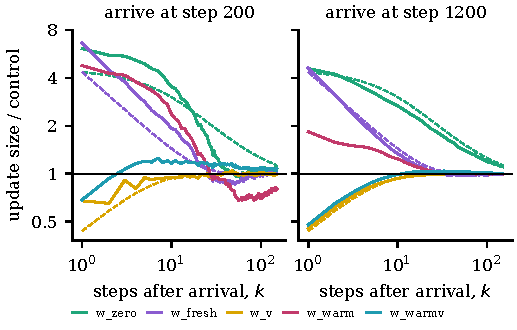
\includegraphics[width=\columnwidth]{trace}}{}
\caption{Size of each update after arrival, divided by the size of the same update in the uninterrupted run
(\traceScale, mean of \traceSeeds{} seeds). Dashed lines are the noise-dominated column of
Proposition~\ref{prop:transient}, with no fitted parameter.}
\label{fig:trace}
\end{figure}

\textbf{Measured update sizes.} Fig.~\ref{fig:trace} overlays the prediction on the measured size of every update for
the first \traceSteps{} steps after arrival.
At 60\% of the schedule the closed forms follow the measurement from the first step to the last. With both moments
zeroed and the counter kept, the first update is \traceZeroOne{} times the control's (predicted \predZeroOne), the
tenth \traceZeroTen{} (\predZeroTen) and the hundredth still \traceZeroHundred{} (\predZeroHundred). With the counter
reset the first update is the same size, \traceFreshOne, and the tenth is down to \traceFreshTen{} (\predFreshTen);
by the hundredth it is \traceFreshHundred. With only $m$ dropped the first update is \traceVOne{} of the control's
(\predVOne) and the tenth \traceVTen{} (\predVTen); the rank-one sketch of $v$ gives \traceRankOne{} and
\traceRankTen, indistinguishable from the exact $v$, and the quantised moments give \traceQOne{} throughout.
At 10\% of the schedule, where the learning rate is at its peak and the loss is still falling fast, the gradient is not
pure noise and the weights move during the transient; the initial inflation is larger than the noise-dominated
value (\traceZeroOneEarly{} and \traceFreshOneEarly) and the run with the kept counter falls back to the control's
step size sooner than predicted, after the damage of Section~\ref{sec:fork} is done. The ordering of the strategies is
the same at both points.


\textbf{A first moment cannot be re-estimated at a point.} The \arm{warm} rule rebuilds $m$ as the mean of
\warmPasses{} gradients at the arrival weights. Under the model above this would have nearly the same size as the
carried $m$, since averaging \warmPasses{} independent gradients removes about as much noise as the exponential average
does. It does not: the rebuilt $m$ is \mnormWarm{} times larger than the one left behind (Section~\ref{sec:diag}). The
model's assumption of independent gradients is what fails. Along a training trajectory successive gradients are
anti-correlated in the directions of high curvature, where adaptive methods oscillate~\cite{cohen2022aeos}, and the
exponential average cancels them. Gradients taken repeatedly at one point all contain that component with the same
sign. The moment $m$ is therefore a statistic of the trajectory and not of the point where it stopped, and an estimate
made at a standstill overstates it. Squared gradients do not cancel, so $v$ can be re-estimated at a point; that is
the \arm{warmv} rule.

\section{Experimental Method}
\label{sec:setup}

\subsection{One variable}
\label{sec:determinism}

A migrated run and its control must differ only in the state that crossed. Three mechanisms enforce this. The batch
used at step $t$ is drawn from a generator seeded by a hash of the run seed, the stream and $t$, so the data order is a
function of the step index and no loader state exists to be restored incorrectly. Dropout masks are seeded the same
way. The learning rate is a function of $t$. Training, the destination's warm-up passes and held-out evaluation use
three separate streams, so the warm-up passes neither consume nor repeat training batches. Deterministic kernels are
enforced in the framework. Under these conditions a migration with the \arm{full} strategy reproduces the control's
loss at every later step bit for bit, on the same device; the test suite asserts this, and \arm{full} appears in the
tables as a row of exact zeros. This is the bitwise standard EasyScale sets for elastic
training~\cite{li2023easyscale}, used here as an instrument: any gap in any other row was caused by the missing
state.

Each control saves a full snapshot at every migration point. A migration cell loads the snapshot into a source
process, packs the strategy's payload, writes it, reads it into a freshly built destination, rebuilds what is missing
and trains for $W = \horizon$ further steps. Nothing but the bundle passes from one to the other.

\subsection{Metrics}

Loss is evaluated every \evalEvery{} steps on a fixed held-out set of \evalSamples{} sequences. Training loss is too
noisy at these sizes and is confounded with which batch lands on which step. Let $L_{\mathrm{mig}}$ and
$L_{\mathrm{ctrl}}$ be the held-out losses of a migrated run and of its own control, with the same seed, and
$\Delta(j) = L_{\mathrm{mig}}(T+j) - L_{\mathrm{ctrl}}(T+j)$.

\textbf{Seed band.} For each model size and migration point, $\eps$ is the 95th percentile of
$|L_a(t) - L_b(t)|$ over all pairs of control seeds $a \ne b$ and all evaluations in $(T, T+W]$. It measures how far
apart two runs of the same job are for no reason at all. A migrated run with $\Delta \le \eps$ is no further from its
control than another seed would be. With \nSeedsMax{} seeds there are three such pairs at each point, so the band is
a coarse estimate; across the sweep it lies between \epsMin{} and \epsMax\mnats.

\textbf{Peak excess loss} is $\max_j \Delta(j)$, reported in thousandths of a nat (mnats) and as a multiple of $\eps$.
It is the main quantity in the tables because it is defined for every run and has a direct reading: a ratio below one
means the run never left the band.

\textbf{Steps to recovery} (StR) is the first offset $k$ such that $\Delta(j) \le \eps$ for all $j \in [k, k+50]$.
One lucky crossing does not count. A run with no such $k$ inside the window is censored and reported as $>W$; it is
never assigned the window length. Tables give the number of runs with $\mathrm{StR} = 0$, which never left the band,
the median StR of those that left and returned, and the number censored.

\textbf{Regret} is $\sum_j \max(0, \Delta(j))$ over the window, in nat-steps. It separates a deep, brief transient from
a shallow, long one.

\textbf{Steps lost} converts the training-loss gap at the end of the window into the number of steps by which the
migrated run trails its control, read off the control's smoothed loss curve, plus any warm-up passes spent. It is the
unit a scheduler wants, and it is noisy: applied to pairs of controls it gives values of \bandLamMin{} to
\bandLamMax{} steps with no migration at all. We report it with that caveat and use it only in the cost model.

\textbf{Uncertainty.} The migration points of one seed share a control and are not independent. Intervals are
therefore 95\% percentile intervals from \bootDraws{} bootstrap resamples of whole seeds.

\subsection{Workloads and hardware}

The main workload is a decoder-only transformer trained on character-level text~\cite{karpathy2022nanogpt} at three
sizes, \paramsXS{}M, \paramsS{}M and \paramsM{}M parameters, for \maxSteps{} steps with AdamW, $\beta_1 = 0.9$,
$\beta_2 = 0.99$, weight decay 0.1, gradient clipping at 1, a \warmupSteps-step warm-up and cosine decay, batch 64 and
context 256, under bfloat16 autocast with single-precision master weights and moments. Each size is run with
\nSeedsMax{} seeds and migrated at steps \forkList{}, that is, 10\%, 30\%, 60\% and 85\% of the schedule. A second sweep repeats nine of the strategies on the middle size at
$\beta_2 = 0.95$ and $0.999$, with migrations at 10\% and 60\% (Section~\ref{sec:beta}), and a twelve-layer model of \largeParams{}M parameters is
run with five strategies at the same two points (Section~\ref{sec:large}).

All but one experiment ran on one laptop: an Intel Core Ultra 9 185H with 32\,GB of memory, an NVIDIA RTX 4050 Laptop GPU with
6\,GB, and the processor's integrated Arc GPU, under Windows 11 with PyTorch 2.14 (CUDA 12.6) and, for the integrated
GPU, PyTorch 2.15. The one exception is the remote resume of Section~\ref{sec:device}, which ran on an NVIDIA T4 in a
hosted notebook under Linux with PyTorch 2.11. Every run writes a manifest with the commit, the resolved configuration, the device, the measured
payload size and the median step time.

\section{Results}
\label{sec:results}

\begin{table*}[t]
\caption{Cost of each strategy. Top: the \paramsM{}M-parameter model, all migration points and \seedsM{} seeds.
Middle: the \largeParams{}M-parameter model (\largeSeeds{} seeds, two migration points). Bottom: ResNet-18 on CIFAR-10
(\cifarSeeds{} seeds). Payload is the share of the full state's bytes. Peak is the largest excess held-out loss in
the \horizon{} steps after arrival; Peak/$\eps$ divides it by the seed band of the same cell, so values below one are
inside the noise floor. Brackets are 95\% seed-bootstrap intervals. StR\,$=0$ counts runs that never left the band; StR
is the median recovery time, in steps, of those that left and returned; $>\!W$ counts runs still outside at the end of
the window.}
\label{tab:main}
\centering
\footnotesize
\begin{tabular}{@{}lrrrrrccc@{}}
\toprule
Strategy & Payload\,\% & Peak (mnats) & Peak/$\eps$ & Regret (nat-steps) & Steps lost & StR\,$=0$ & StR & $>\!W$ \\
\midrule
\gen{tab_main}
\midrule
\gen{tab_large}
\midrule
\gen{tab_cifar}
\bottomrule
\end{tabular}
\end{table*}

\begin{figure*}[t]
\centering
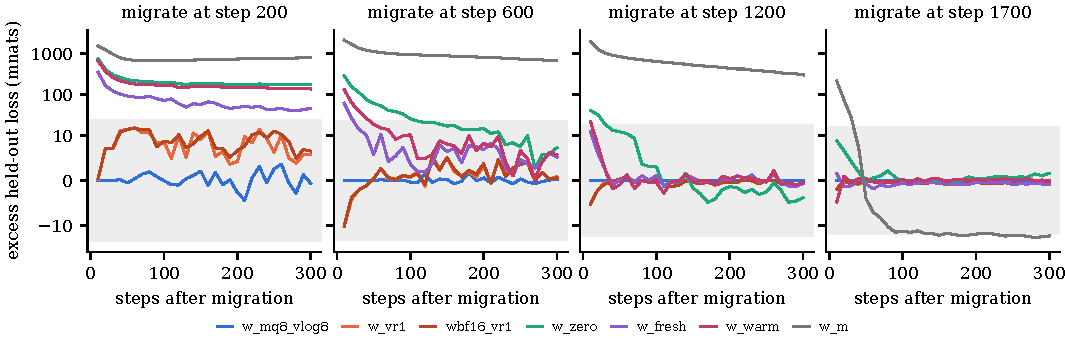
\includegraphics[width=\textwidth]{curves}
\caption{Excess held-out loss after a migration at four points in training (\paramsM{}M parameters, mean over seeds;
the vertical axis is linear within $\pm10$\mnats{} and logarithmic outside). The grey band is $\pm\eps$, the spread
between seeds of the uninterrupted run.}
\label{fig:curves}
\end{figure*}

\subsection{What must cross}
\label{sec:main}

Pending.


\begin{figure*}[t]
\centering
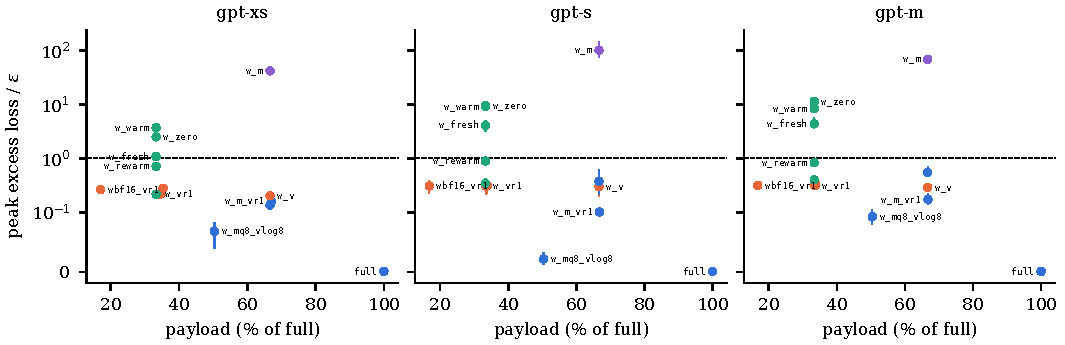
\includegraphics[width=\textwidth]{frontier}
\caption{Bytes against damage at the three model sizes. Each point is a strategy; the horizontal axis is its payload
as a share of the full state, the vertical axis its peak excess loss in units of the seed band, with 95\% intervals.
The dashed line is the noise floor.}
\label{fig:frontier}
\end{figure*}

\begin{table*}[t]
\caption{Peak excess held-out loss in mnats by migration point (\paramsM{}M parameters), with the seed band of each
point in the first row.}
\label{tab:fork}
\centering
\footnotesize
\begin{tabular}{@{}lrrrr@{}}
\toprule
Strategy & Step 200 (10\%) & Step 600 (30\%) & Step 1200 (60\%) & Step 1700 (85\%) \\
\midrule
\gen{tab_fork}
\bottomrule
\end{tabular}
\end{table*}

\subsection{When it matters}
\label{sec:fork}

Pending.


\subsection{First-update diagnostics}
\label{sec:diag}

\begin{table}[t]
\caption{The first update after arrival against the true one (\paramsM{}M, mean over migration points). cos: cosine
with the control's update. Size: norm ratio. $|m|$: norm of the installed first moment over the true one.
$\sqrt{v}$ err: median relative error of the installed $\sqrt{v}$, in percent. The last four columns split cosine and
error into matrices (mat.) and embedding tensors (emb.).}
\label{tab:diag}
\centering
\footnotesize
\setlength{\tabcolsep}{2.6pt}
\begin{tabular}{@{}lrrrrrrrr@{}}
\toprule
 & & & & & \multicolumn{2}{c}{cos} & \multicolumn{2}{c}{$\sqrt{v}$ err} \\
\cmidrule(lr){6-7}\cmidrule(l){8-9}
Strategy & cos & Size & $|m|$ & $\sqrt{v}$ err & mat. & emb. & mat. & emb. \\
\midrule
\gen{tab_diag}
\bottomrule
\end{tabular}
\end{table}

Pending.


\subsection{Sensitivity to the second-moment horizon}
\label{sec:beta}

\begin{table*}[t]
\caption{Peak excess loss over the seed band at three values of $\beta_2$ (\paramsS{}M parameters, migration at 10\% and
60\% of the schedule; \betaSeeds{} seeds for the outer columns). Each value is followed by the number of runs that never
left the band.}
\label{tab:beta}
\centering
\footnotesize
\begin{tabular}{@{}lrcrcrc@{}}
\toprule
 & \multicolumn{2}{c}{$\beta_2 = 0.95$} & \multicolumn{2}{c}{$\beta_2 = 0.99$} & \multicolumn{2}{c}{$\beta_2 = 0.999$} \\
\cmidrule(lr){2-3}\cmidrule(lr){4-5}\cmidrule(l){6-7}
Strategy & Peak/$\eps$ & StR\,$=0$ & Peak/$\eps$ & StR\,$=0$ & Peak/$\eps$ & StR\,$=0$ \\
\midrule
\gen{tab_beta}
\bottomrule
\end{tabular}
\end{table*}

Pending.


\subsection{Drain and restore latency}
\label{sec:latency}

\begin{table*}[t]
\caption{Latency of one migration in milliseconds on the discrete GPU (\paramsM{}M parameters, median of \latReps{}
rounds after warm-up rounds; brackets are the 5th and 95th percentiles). Drain is everything the source does inside the
notice window; restore is everything the destination does before its first step.}
\label{tab:latency}
\centering
\footnotesize
\setlength{\tabcolsep}{4pt}
\begin{tabular}{@{}lrrrrrrrrrrr@{}}
\toprule
 & & \multicolumn{5}{c}{Drain (source)} & \multicolumn{5}{c}{Restore (destination)} \\
\cmidrule(lr){3-7}\cmidrule(l){8-12}
Strategy & MB & encode & to host & serialise & write & total & read & to device & decode & rebuild & total \\
\midrule
\gen{tab_latency}
\bottomrule
\end{tabular}
\end{table*}

Pending.


\subsection{Across device classes}
\label{sec:device}

\begin{table}[t]
\caption{The \arm{full} payload, written on the discrete GPU, resumed on other devices. Gaps are held-out loss
against the same payload resumed on the discrete GPU, in mnats, over 200 steps. \texttt{fp32\_nodrop}: single
precision, no dropout. \texttt{as\_trained}: bfloat16 autocast and dropout, as in the main sweep.}
\label{tab:device}
\centering
\footnotesize
\setlength{\tabcolsep}{2.8pt}
\begin{tabular}{@{}lrllrrrrr@{}}
\toprule
Model & Step & Device & Condition & Arrival & Mean & Max & $\eps$ & Max/$\eps$ \\
\midrule
\gen{tab_device}
\bottomrule
\end{tabular}
\end{table}

Pending.


\subsection{End-to-end preemption}
\label{sec:chaos}

\begin{table*}[t]
\caption{Injected preemptions and crashes during one training run on the discrete GPU. A preemption drains
\arm{w\_vr1} on notice; a crash falls back to the last periodic \arm{w\_mq8\_vlog8} checkpoint. Times in seconds unless
marked.}
\label{tab:chaos}
\centering
\footnotesize
\begin{tabular}{@{}lrlrrrrrrrr@{}}
\toprule
Event & Step & World & Steps redone & Payload (MB) & Drain & Restart & Init & Fetch (ms) & Rebuild (ms) & Downtime \\
\midrule
\gen{tab_chaos_gpu}
\bottomrule
\end{tabular}
\end{table*}

Pending.


\section{From Measurements to a Migration Policy}
\label{sec:policy}

A scheduler deciding what to send needs three numbers per strategy: its bytes, whether those bytes drain in time, and
what the destination pays to recover. The first is exact for any architecture, since payload size depends only on
tensor shapes and codecs (Table~\ref{tab:bytes}). The second follows from the bandwidth. The third is what we
measured.

\textbf{Model.} Let a strategy $s$ have payload $B_s$ bytes and cost $\lambda_s$ steps of lost progress, and let the
job have bandwidth $w$, notice window $N$, step time $\tau$, $G$ accelerators at price $p$ per accelerator-hour, and
egress price $e$ per gigabyte. The drain takes $x_s = B_s / w$. If $x_s > N$ the payload does not leave in time; the
job restarts from its last periodic checkpoint and loses, in expectation, half a checkpoint interval. Otherwise the
migration costs
\begin{equation}
C_s = e\,B_s + G\,p\,(x_s + \lambda_s \tau),
\label{eq:cost}
\end{equation}
bytes on the wire plus accelerators idle during the drain and busy re-earning lost progress. The policy picks the
feasible strategy with the lowest $C_s$. A job that moves by choice, toward a cheaper region, moves only if the price
difference over its remaining steps exceeds $C_s$.

\textbf{An illustrative case.} Table~\ref{tab:policy} applies the model to the shapes of a \llamaParams{}-billion
parameter decoder~\cite{touvron2023llama2} with $G = 8$, $p = \$1.20$, $\tau = 6$\,s, $e = \$0.02$ per gigabyte and a
checkpoint every 1000 steps. \emph{These rows are extrapolations.} The byte counts are exact for those shapes. The
values of $\lambda_s$ are those measured at \paramsM{}M parameters for a migration at 60\% of the schedule, held
constant, and nothing here was trained at
that size. With that caveat the structure of the answer is robust to the exact $\lambda_s$, because it is driven by
feasibility. The full state, \llamaFullGB{}\,GB, needs \llamaFullDrain{}\,s at 10\,Gb/s. It fits a two-minute notice and
misses a thirty-second one, where a job that insists on it is thrown back to its last checkpoint. The quantised state
(\llamaQGB{}\,GB, \llamaQDrain{}\,s) still misses. The rank-one strategies (\llamaRankGB{}\,GB in \llamaRankDrain{}\,s,
or \llamaRankBfGB{}\,GB in \llamaRankBfDrain{}\,s with half-precision weights) fit with room to spare, and are the
ones Section~\ref{sec:main} found inside the noise floor. Fig.~\ref{fig:policy} shows the same boundary across
bandwidths.

\begin{table*}[t]
\caption{Policy output for a \llamaParams{}-billion-parameter model. \textbf{Extrapolated}: payload sizes are computed
from tensor shapes; recovery costs are those measured at \paramsM{}M parameters. Drain times are bytes over bandwidth
and exclude encoding.}
\label{tab:policy}
\centering
\footnotesize
\begin{tabular}{@{}lrrrcclrrr@{}}
\toprule
 & & & \multicolumn{2}{c}{\arm{full}} & & \multicolumn{4}{c}{Chosen strategy} \\
\cmidrule(lr){4-5}\cmidrule(l){7-10}
Scenario & Notice (s) & Gb/s & Drain (s) & Fits & Strategies that fit & Name & GB & Drain (s) & Cost (\$) \\
\midrule
\gen{tab_policy}
\bottomrule
\end{tabular}
\end{table*}

\begin{figure}[t]
\centering
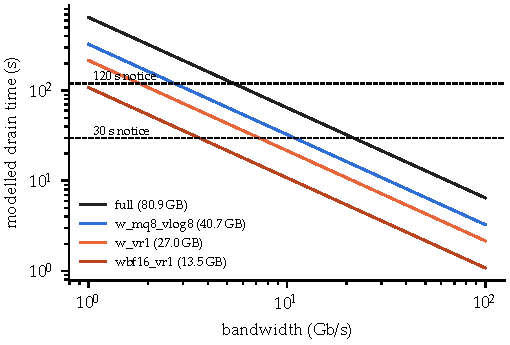
\includegraphics[width=\columnwidth]{policy}
\caption{Modelled drain time of four payloads for a \llamaParams{}-billion-parameter model against bandwidth
(extrapolated from tensor shapes; not measured). A payload above a dashed line does not leave within that notice.}
\label{fig:policy}
\end{figure}

\textbf{Reading the measurements as a rule.} Combined with Sections~\ref{sec:main}--\ref{sec:diag}, the policy reduces
to an order of preference. Send the quantised moments if they fit, since they cost nothing measurable. Otherwise drop
$m$ and send the rank-one sketch of $v$, with the weights in half precision if the window is still too short. If only
the weights can leave, the destination should re-estimate the second moment with a few frozen passes and leave the
first at zero, or, if it cannot spare the passes, build a new optimizer and ramp the learning rate again. It should not
keep the step counter over empty moments, and it should not re-estimate the first moment. Late in training the choice hardly matters and the smallest payload is the right
one; early in training it matters most (Section~\ref{sec:fork}).

\section{Limitations}
\label{sec:limits}

\textbf{Scale.} The largest model trained is \largeParams{}M parameters, with five strategies at two migration points;
the full sweep stops at \paramsM{}M. Everything ran on one laptop GPU and one small text dataset. The
mechanisms of Section~\ref{sec:transient} depend only on the decay rates and are not specific to a size, and the
measured picture is stable across a factor of a hundred in parameter count (Fig.~\ref{fig:frontier},
Section~\ref{sec:large}), but none of this
is evidence about a multi-billion-parameter run. Every figure quoted for such a model is an extrapolation and is
labelled.

\textbf{Three seeds.} Each cell has \nSeedsMax{} seeds, so each seed band is the 95th percentile over three pairs of
controls and each interval resamples three units. The three groups of strategies are separated by more than an order
of magnitude, which three seeds resolve; the differences inside a group, such as rank one against rank four, are not
resolved and we do not claim them. The dependence on $\beta_2$ was measured at one model size and two migration
points, and $\beta_1$ was not varied. The vocabulary is a few dozen characters, so the embedding results do not transfer to a
tokenised model.

\textbf{Simulated transport.} A migration here serialises to local storage, tears the model and optimizer down and
rebuilds them from the bundle. That reproduces exactly the information lost by a real migration, which is what the
loss measurements depend on. It does not reproduce a network: the drain times in Section~\ref{sec:policy} are bytes
divided by an assumed bandwidth, and the measured latencies of Section~\ref{sec:latency} cover encoding and local I/O
only. Section~\ref{sec:link} sends payloads between two processes through a paced socket, which reproduces a
bandwidth and not a network: there is no loss, jitter or competing traffic. Payloads were also resumed on a second
machine (Section~\ref{sec:device}), but that transfer was not timed. A timed migration between two machines over a real
link has not been run.

\textbf{One host.} The multi-rank runtime was exercised with CPU ranks on one machine over Gloo. Resizing a job changes
its world size, not its node count, and no claim is made about a GPU cluster.

\textbf{Device classes.} Four trainable devices were tested: an x86 CPU, an NVIDIA laptop GPU, an Intel integrated GPU
and an NVIDIA T4 on a second machine.
The laptop also has a neural processing unit, and it was not used: current NPU software stacks execute inference
graphs and offer no backward pass~\cite{openvino2025npu,feng2024steppingforward}, so a training job cannot be migrated
to one. No TPU run was made. The integrated-GPU and remote-GPU runs use other framework releases than the
rest, so those rows change device and framework version together.

\textbf{One optimizer family.} All runs use AdamW. The analysis carries over to any method built on the same two
exponential averages; it says nothing about second-order or sign-based methods, or about schedules with restarts.

\textbf{Sharded state.} Rank zero drains the whole payload. With tensor- or pipeline-parallel training the state is
partitioned across devices and each shard would drain its own part; the strategies apply per tensor and do not depend
on where a tensor lives, but that path was not built.

\textbf{Steps lost.} The cost model's $\lambda_s$ comes from training loss and has a wide noise band. The peak, regret
and recovery measures on held-out loss are the reliable ones, and our conclusions rest on those.

\textbf{Concurrent work.} The literature search was last run in November 2026. The two closest preprints are discussed
in Section~\ref{sec:related}; others may have appeared since.

\section{Conclusion}
\label{sec:conclusion}

Systems for preemptible training have treated Adam's state as indivisible and the cost of recovering from a move as a
constant. Measured against a bit-identical control and a seed-to-seed noise floor, the state divides cleanly. The first
moment is a ten-step memory and can be left behind. The second moment is needed only as a per-tensor scale, which its
row and column sums supply in a hundredth of a percent of its bytes. The step counter belongs with the moments: kept
with empty moments it does harm. A first moment cannot be rebuilt at the destination, because it records the path and
not the place. Each of these statements is a prediction of a two-line model of the update and each is borne out by the
measurements.

For a scheduler the consequence is that the changeover delay is a choice. A third or a sixth of the bytes buys a
transient that cannot be told from a change of seed, and that turns a notice window which the full state misses into
one that is met several times over. The measurements here stop at \largeParams{}M parameters and one machine. The
method does not: a deterministic control, a seed band and a censored recovery time are cheap to reproduce on any
cluster, and the open question, whether the same curve holds at the sizes where the bytes hurt, is one experiment for
anyone who has the hardware.


\section*{Data and Code Availability}
The implementation, every experiment configuration, the per-run manifests, the raw loss series and the scripts that
regenerate each table, figure and in-text number of this paper from those series are available at
\url{https://github.com/riteshroshann/minstate}. No number in the paper is typed by hand: the manuscript inputs a
generated macro file.

\section*{Acknowledgment}
The author thanks the School of Artificial Intelligence, Amrita Vishwa Vidyapeetham, for its support. All experiments ran
on the author's own laptop; no external compute grant was used.

\bibliographystyle{IEEEtran}
{\raggedright\small
\bibliography{refs}}

\begin{IEEEbiographynophoto}{Ritesh Roshan Sahoo}
is with the School of Artificial Intelligence, Amrita Vishwa Vidyapeetham, Faridabad, India. His research
interests are distributed training systems, optimization for deep learning and high-performance computing.
\end{IEEEbiographynophoto}

\end{document}
